\documentclass{article}

% Language setting
% Replace `english' with e.g. `spanish' to change the document language
\usepackage[english]{babel}

% Set page size and margins
% Replace `letterpaper' with `a4paper' for UK/EU standard size
\usepackage[letterpaper,top=2cm,bottom=2cm,left=3cm,right=3cm,marginparwidth=1.75cm]{geometry}

% Useful packages
\usepackage{amsmath}
\usepackage{graphicx}
\usepackage[colorlinks=true, allcolors=blue]{hyperref}
\usepackage{float}


\title{Poisonous or Edible Mushroom?}
\author{Campregher Sofia}

\begin{document}
\maketitle


\begin{abstract}
This project presents a custom decision tree which is implemented entirely from scratch, using only single-feature binary tests at each internal node. 
Firstly, the dataset is processed in order to handle and encode missing values; columns with more than 50% missing data are removed, while the remaining missing values are replaced using each mode.

The initial static analysis focuses on building a constructor which only accepts one of the following impurity measures - Gini Index, Entropy, or Scaled Entropy as the metric for evaluating splits, while all the other parameters are fixed. The highest Test Accuracy is reached by the Gini index model. Both Entropy and Scaled Entropy yielded identical test accuracy and zero-one loss scores.
The Gini index offers a small advantage in terms of classification accuracy.
The computational costs, given the manual implementation, are analyzed by the Training time analysis; where Gini required 65.64 seconds, and Entropy and Scaled Entropy 58.59 and 57.58 seconds, respectively.

The model performed a hyperparameter tuning that is implemented by varying the maximum depth from [3,9] and following a different splitting criterion. The optimal configuration is obtained using the Gini index as a splitting criterion and a maximum depth of 9. This model recorded a training test accuracy of 0.839201 and an overfitting gap of just 0.000079; showing no signs of overfitting. Both Entropy and Scaled Entropy reached a maximum test accuracy of 0.799.

Performance is visualized by a heat map that displays test accuracy as a function of the maximum depth and the splitting criterion used in the decision tree. The test accuracy decreases as the maximum depth of the tree decreases, which means that trees of a lower depth are less effective in capturing the complexity of the data set across all three parameters. Overall, the project demonstrates that despite the high computational costs, a model implemented from scratch can achieve great results in terms of accuracy.
\end{abstract}

\section{Introduction}

The decision tree aims to create a model that estimates the value of a target variable by learning decision rules derived from the features of the dataset. 
This technique is widely used because of:
\begin{itemize}
    \item Its simplicity to understand and interpret
    \item It requires little data preparation
    \item It is able to handle both numerical and categorical data
    \item It performs well on large datasets
\end{itemize}
This project offers a custom decision tree which is implemented entirely from scratch, using only single-feature binary tests at each internal node. The initial static analysis focuses on building a class structor which contains several parameters which control the behavior and growth of the model. The constructor accepts one of the following impurity measures, Gini index, entropy, or scaled entropy, as the metric for evaluating splits, while others parameters are fixed.
The model performs a hyperparameter tuning which is implemented to assess how the adoption of different combinations of splitting criteria and maximum tree depth influence accuracy and generalization. In the last section of the study, training and test set are analyzed using accuracy scores, overfitting gap, and confusion matrices to draw conclusion about its performance.

\section{DataSet}
\subsection{Mushroom Dataset Overview}
The Mushroom Dataset is made up of a collection of 61,068 instances, hypothetical mushroom entities, one class, and 20 attributes, which describe the properties of mushrooms; each instance is represented by a set of features. All these features, used to train the model, can be categorical or continuous [17 nominal and 3 metrical] and describe various physical and chemical attributes of mushrooms. 
Below, a sample of several attributes included in the dataset: 
\begin{itemize}
    \item Cap Shape (e.g., bell, conical, flat)
    \item Cap Surface (e.g., smooth, scaly)
    \item Cap Color (e.g., red, green, yellow)
    \item Bruises (whether the mushroom bruises when handled)
    \item Odor (e.g., almond, anise, foul, none)
    \item Gill Attachment (e.g., attached, free)
    \item Gill Spacing (e.g., close, crowded)
    \item Gill Size (e.g., narrow, broad)
    \item Stalk Shape (e.g., enlarging, tapering)
    \item Stem Height (float value in cm)
    \item Stem Width (float value in mm)
    \item Cap Diameter (float value in cm)
\end{itemize}


\begin{figure}[H]
\centering
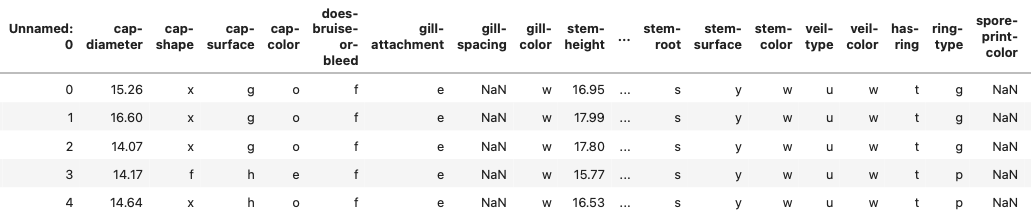
\includegraphics[width=1\linewidth]{Dataset.png}
\caption{\label{fig:frog}Dataset Composition}
\end{figure}


Since and the goal is to predict and to then classify each mushroom as either edible or poisonous based on these features, the target variable for the Mushroom Dataset is a binary classification label:
\begin{itemize}
    \item Edible (represented as e)
    \item Poisonous (represented as p)
\end{itemize}
The data from the UCI Machine Learning Repository is a structured data frame of information; where each column corresponds to a particular feature, and each row represents a mushroom instance.

 The data is split into two parts:
\begin{itemize}
    \item Features (X): the input data, - categorical or continuous features.
    \item Targets (y): the classification label - edible or poisonous.
\end{itemize}

As mentioned before, features can be categorical [eg. cap-shape] or continuous [eg. cap-diameter]. Nominal attributes are encoded, in the row file, as a single letter, instead, metrical attributes are represent as an interval of floats number. The "nan" values indicate missing values and uncoded letter (such as “d” for Cap-Shape) means that the specific one-digit code is absent from the metadata file.

The Dataset includes:
\begin{itemize}
    \item three numerical attributes: cap diameter [avg 6.7 cm], stem height [avg 6.58cm] and stem width[avg 12.5cm];
    \item Missing data in several features: stem root [84.39%], spore print color [89.60%] and veil-type [94.80%]
\end{itemize}

The distribution of categorical variables is displayed by 12 plots. Each of them show the frequency of values for each feature in the dataset, but also detect the dominant classes and potentially underrepresented categories.

\begin{figure}[H]
\centering
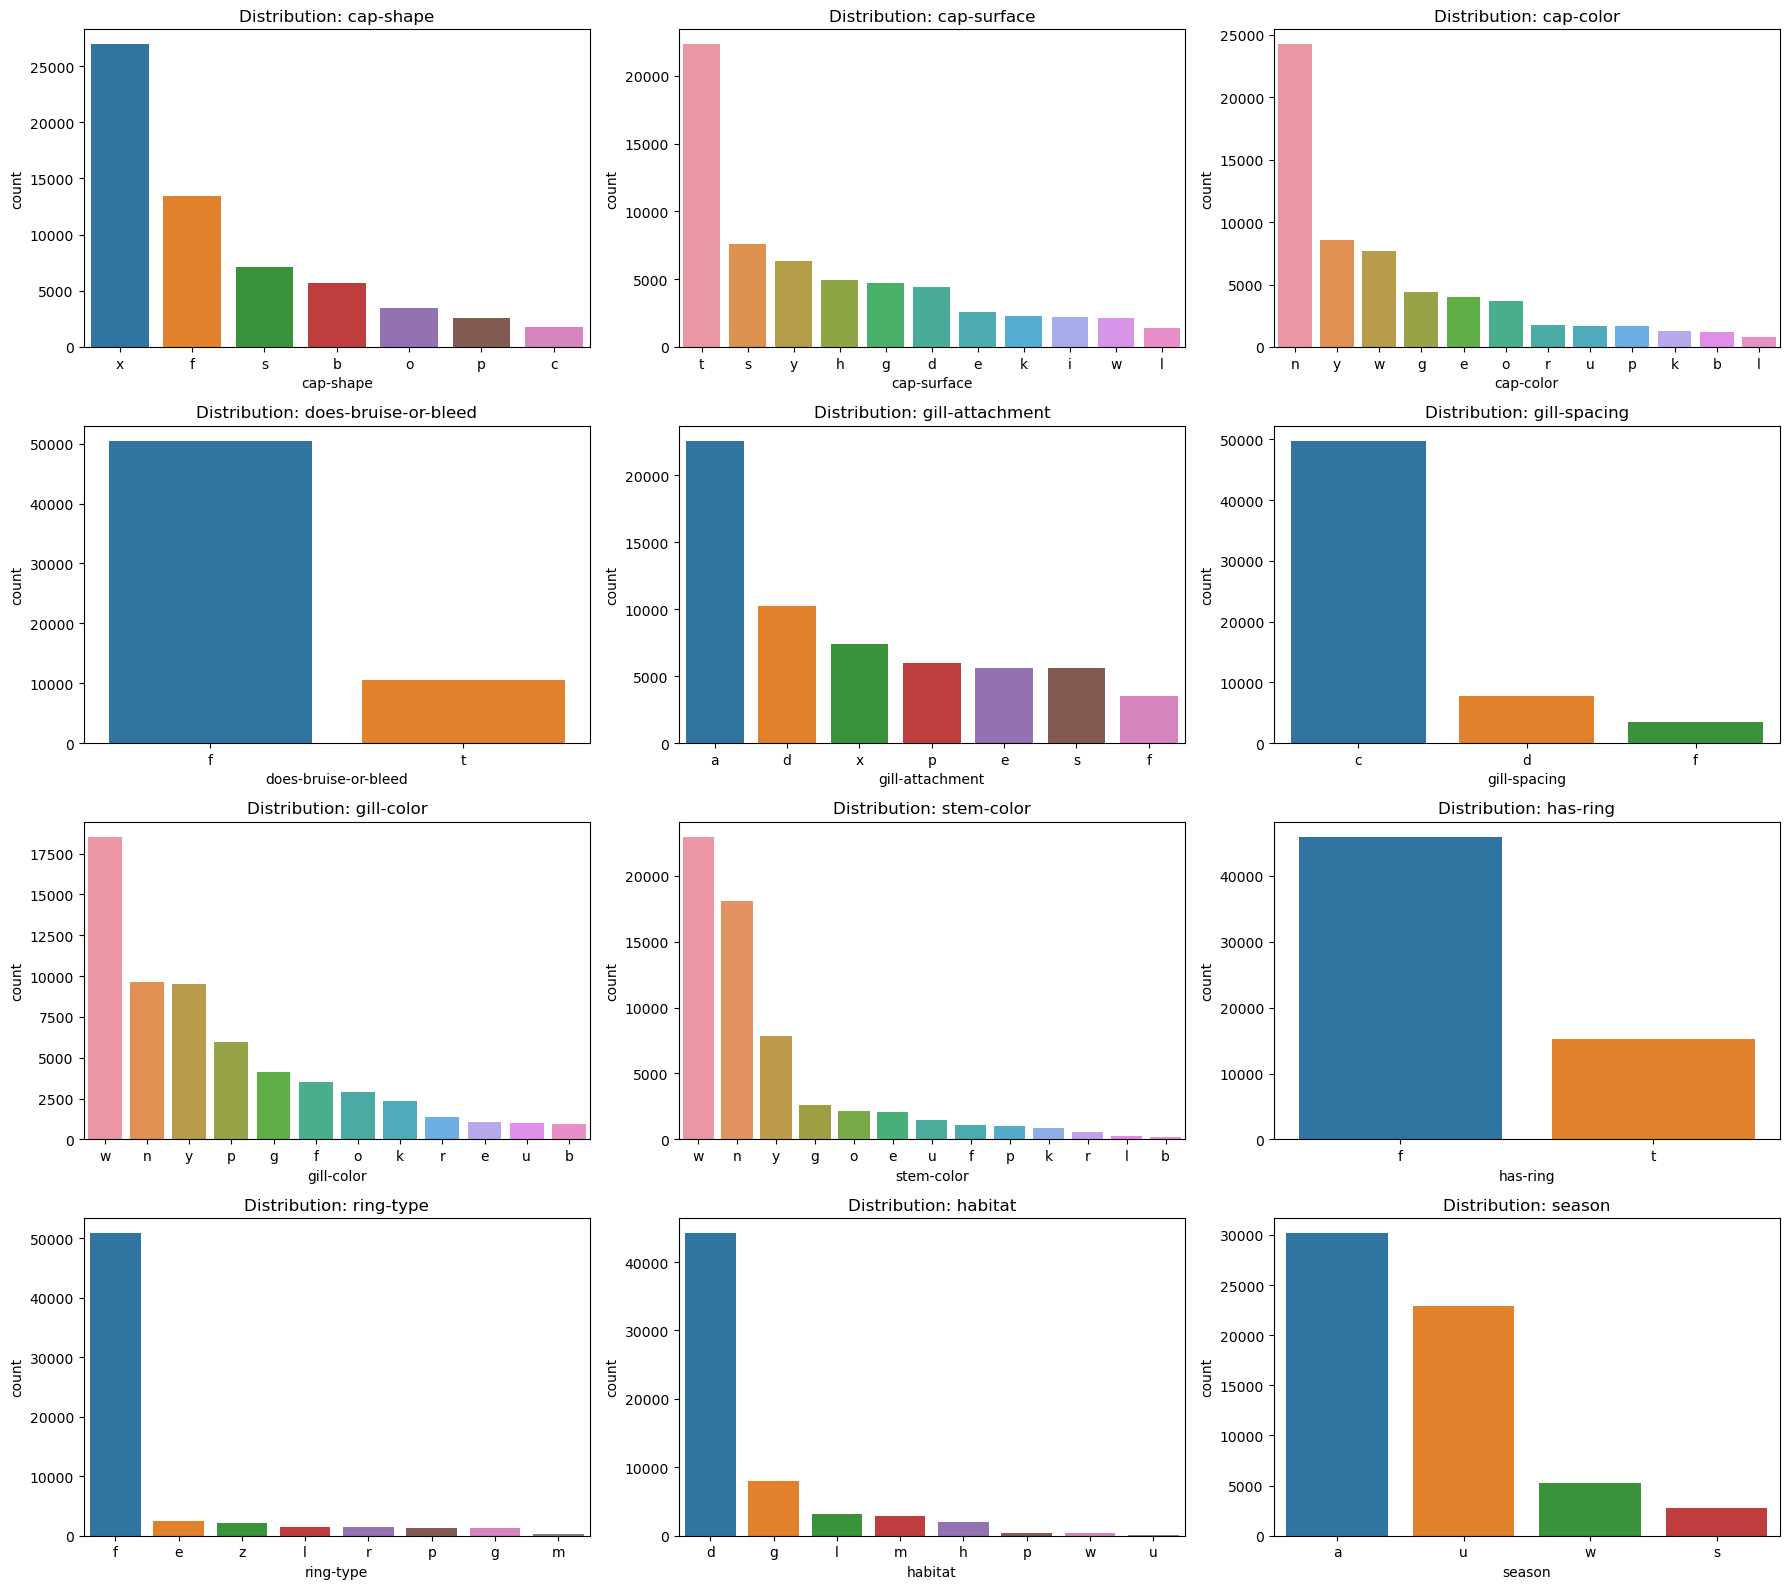
\includegraphics[width=1\linewidth]{Distribution-Cat.png}
\caption{\label{fig:frog}Distribution of categorical features}
\end{figure}

The distribution of numerical variables is explored through histogram plots to asses the shape, tendency, trend and spread of each features. 
Histograms are combined with Kernel Density Estimation (KDE) - which provides approximation of the data distribution. All three variables present a right-skewed distribution, where most observations are concentrated in the lower range values.

\begin{figure}[H]
\centering
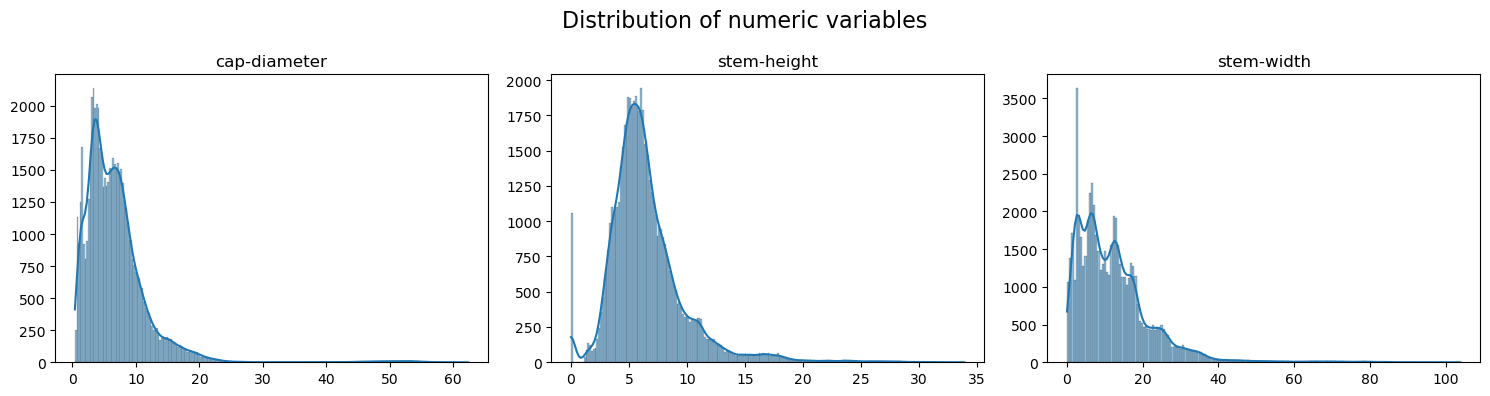
\includegraphics[width=1\linewidth]{Distribution-Num.png}
\caption{\label{fig:frog}Distribution of numerical features}
\end{figure}

The analysis focuses exclusively on the Secondary Mushroom Dataset, as it is more comprehensive and it offered an enriched collection of features. The secondary dataset includes both numerical and categorical features which are not present in the primary. In addition, the secondary data set is a more recent release (2022).  


\subsection{Statistical Property}

The data set is largely balanced; indeed, considering the class distribution, the percentage of mushrooms being poisonous is 55.49% and 44.51% for those considered edible. 

The following heatmap illustrates the correlation matrix for all variables in the dataset, including the target variable - class. All categorical features were encoded into numerical format using integer number. The correlation values are formed by [-1, 1], where -1 means perfect negative correlation and 1 perfect positive correlation. 


\begin{figure}[H]
\centering
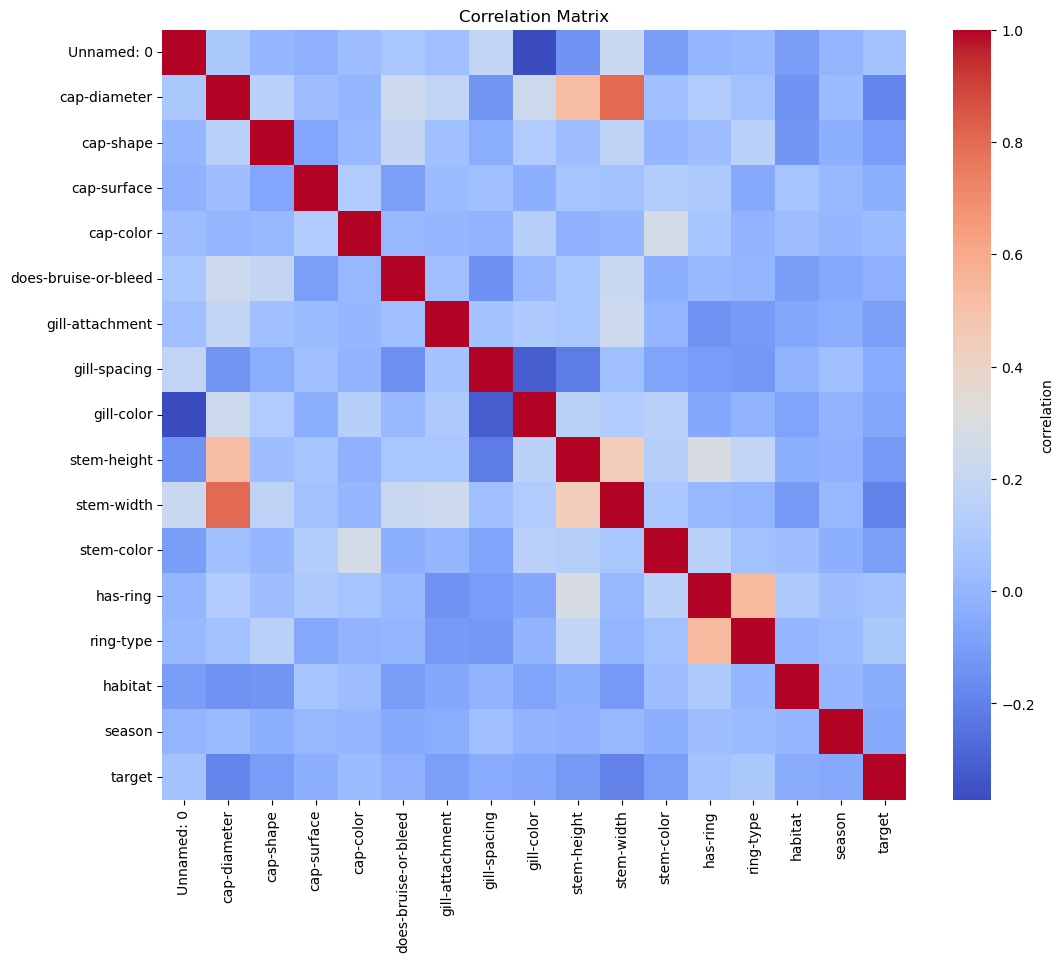
\includegraphics[width=0.5\linewidth]{Correlation-All.png}
\caption{\label{fig:frog}Correlation}
\end{figure}


The diagonal displays a perfect positive correlation for each variable with itself, and off diagonal elements exhibit weak or no correlation. The only couples that exhibits some positive structural dependency are cap-diameter - stem-height, and cap-diameter - stem-width. The target attributes, class - shows very weak correlation with most predictors.

A specific insight into the numerical variable correlation is exhibits by the following heatmap:

\begin{figure}[H]
\centering
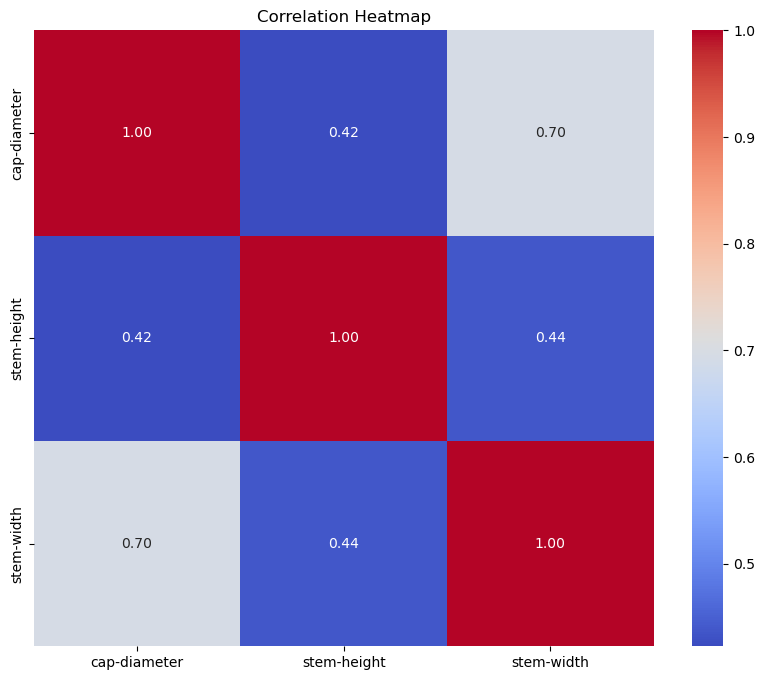
\includegraphics[width=0.30\linewidth]{Correlation-Num.png}
\caption{\label{fig:frog}Correlation of numerical features}
\end{figure}


The annoyed value represents the strength and direction of their linear relationships. The highest is observed by the couple cap-diameter - stem-width, suggesting that mushrooms with larger caps also tend to have thicker stems. A moderate positive and negative correlation is reached by stem height - cap diameter - and stem height - stem width, respectively.

\section{Methodology}

In this section, we describe the methodology behind the decision tree predictor implemented in Python. The model is based on a binary tree structure, where each node represents a decision point. The tree construction follows a recursive splitting approach, using impurity measures such as Gini Impurity, Entropy and Scaled Entropy to evaluate the quality of a split.


\subsection{Data Preparation}

The DataSet, which is downloaded and stored locally to avoid redundant downloads, is returned as a dictionary. 

The first step of the process involves handling and encoding missing values. Since some categorical and numerical attributes contain missing values, columns with more than 50% missing data are removed, while the remaining missing values are replaced using each mode.

The number and percentage of missing values were calculated for each column:

\begin{figure}[H]
\centering
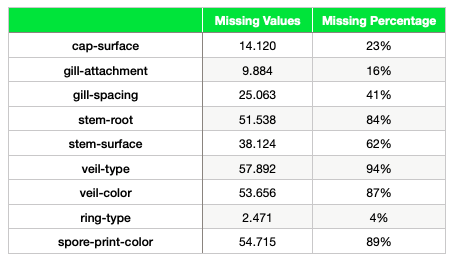
\includegraphics[width=0.7\linewidth]{MissingValue01.png}
\caption{\label{fig:frog}Missing Value and Missing Percentage}
\end{figure}

And visually represented by an horizontal bar plot to display the extent of missingness across features.

\begin{figure}[H]
\centering
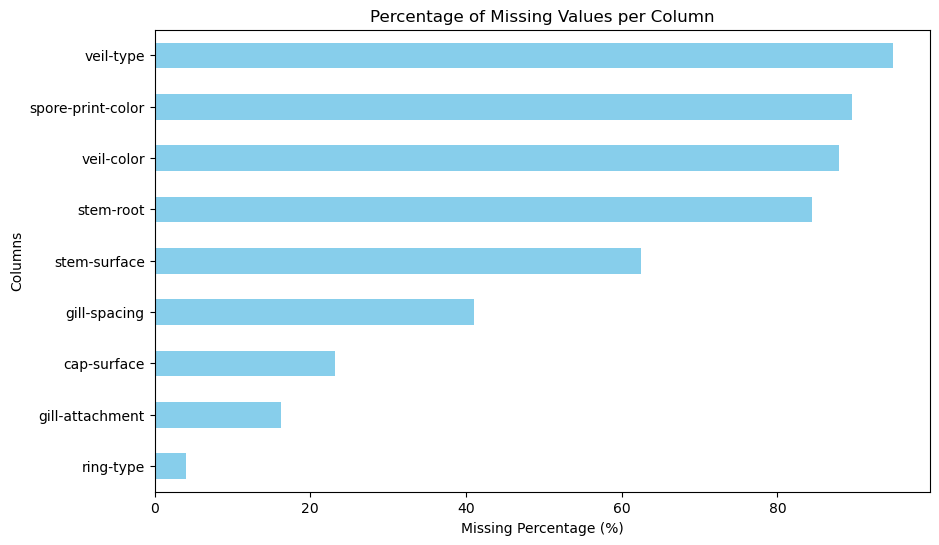
\includegraphics[width=0.7\linewidth]{MissingValue.png}
\caption{\label{fig:frog}Missing Value}
\end{figure}

Columns with more than 50% missing values, which were removed from the dataset, are five. 
Stem-root, Stem-surface, Veil-type, Veil-color, Spore-print-color are considered unreliable.
For the remaining attributes, missing entries are replaced using the mode to preserve categorical consistency. Which are:
\begin{itemize}
    \item t for cap-surface
    \item a for gill-attachment
    \item c for gill-spacing
    \item f for ring-type
\end{itemize}
The mode approach avoids bias might result from mean or median imputation or by dropping the entire column. 

\subsection{Tree Predictors (Theory)}


A tree predictor follows the structure of an ordered, rooted tree where each node could be a leaf or an internal node. The difference between these two is that the first - leaf - does not have any children; on the contrary, the second - internal or test node - has at least two children. The children of each internal node are arranged in a specific sequence, meaning they are indexed consecutively.

An example:

\begin{figure}[H]
\centering
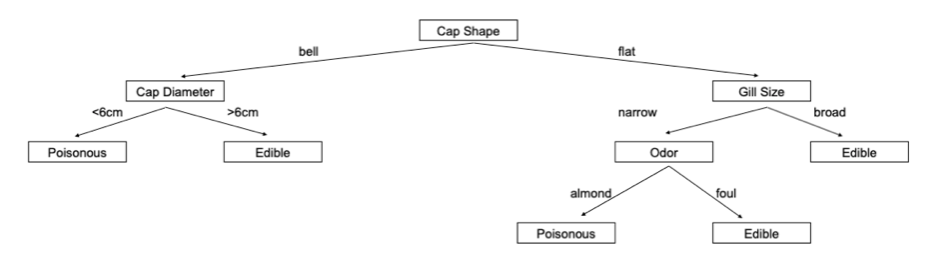
\includegraphics[width=1\linewidth]{TreePredictors.png}
\caption{\label{fig:frog}Tree Predictor}
\end{figure}

The previous decision tree predicts mushrooms editability based on three different attributes: cap shape, cap diameter, gill size and odor. The shape of the cap and the size of the gill are the primary decision factors; the diameter of the cap and the size of the gill are not directly related in the examples; indeed, they are treated as independent risk factors for heart attack. Gill size and odor are linked, indeed when the mushroom present a flat cap shape and a narrow gill size, then the odor could be foul or almond; each of which bring to a different final result.
The three attributes are internal node, where cap shape has three internal nodes and cap diameter and gill size only two. Poisonous and edible are leaf, because, as the image shows, they do not have any children.

Our particular case consider a binary classification where all internal nodes have exactly two children. The process starts with a single node tree, a leaf, which classifies all data point by assigning the most frequent label. The leaf node it is transformed into an internal node from which two new leaves are added. The two new leaves can remain so or can be transformed into internal nodes and restart recursively the model until a stopping condition is met.

\subsection{Impurity Measures (Theory)}

The algorithm used in a decision tree operates aims of minimizing the impurity of the split; in other word, ensuring that the chosen node-question pair (nt,qt) leads to the greatest reduction in impurity according to a given impurity function F. This approach helps prevent overfitting, that is when the number of tree nodes grow to much compared to the cardinality of the training set.
Impurity function must satisfy certain condition, that capture the notion of “impurity”. (Kearns and Mansour, 1999)

The approach used in this paper includes the widely used functions of Entropy, Scaled Entropy and Gini-index.

The following impurity measures are used to evaluate the quality of a split in the decision tree:

\begin{itemize}
    \item \textbf{Standard Entropy:}
    \[
        H(p) = -p \log_2(p) - (1 - p) \log_2(1 - p)
    \]
    Entropy reaches its maximum when $p = 0.5$, indicating maximum uncertainty when both classes are equally likely.

    \item \textbf{Scaled Entropy:}
    \[
        H_{\text{scaled}}(p) = -\frac{p}{2} \log_2(p) - \frac{(1 - p)}{2} \log_2(1 - p)
    \]
    This is a scaled-down version of the standard entropy. It also reaches its maximum value of $0.5$ at $p = 0.5$.

    \item \textbf{Gini Index:}
    \[
        G(p) = 2p(1 - p)
    \]
    Gini Index also peaks at $p = 0.5$, but increases less sharply near the extremes ($p = 0$ or $p = 1$), making it less sensitive to changes in class probability.
\end{itemize}


\begin{figure}[H]
\centering
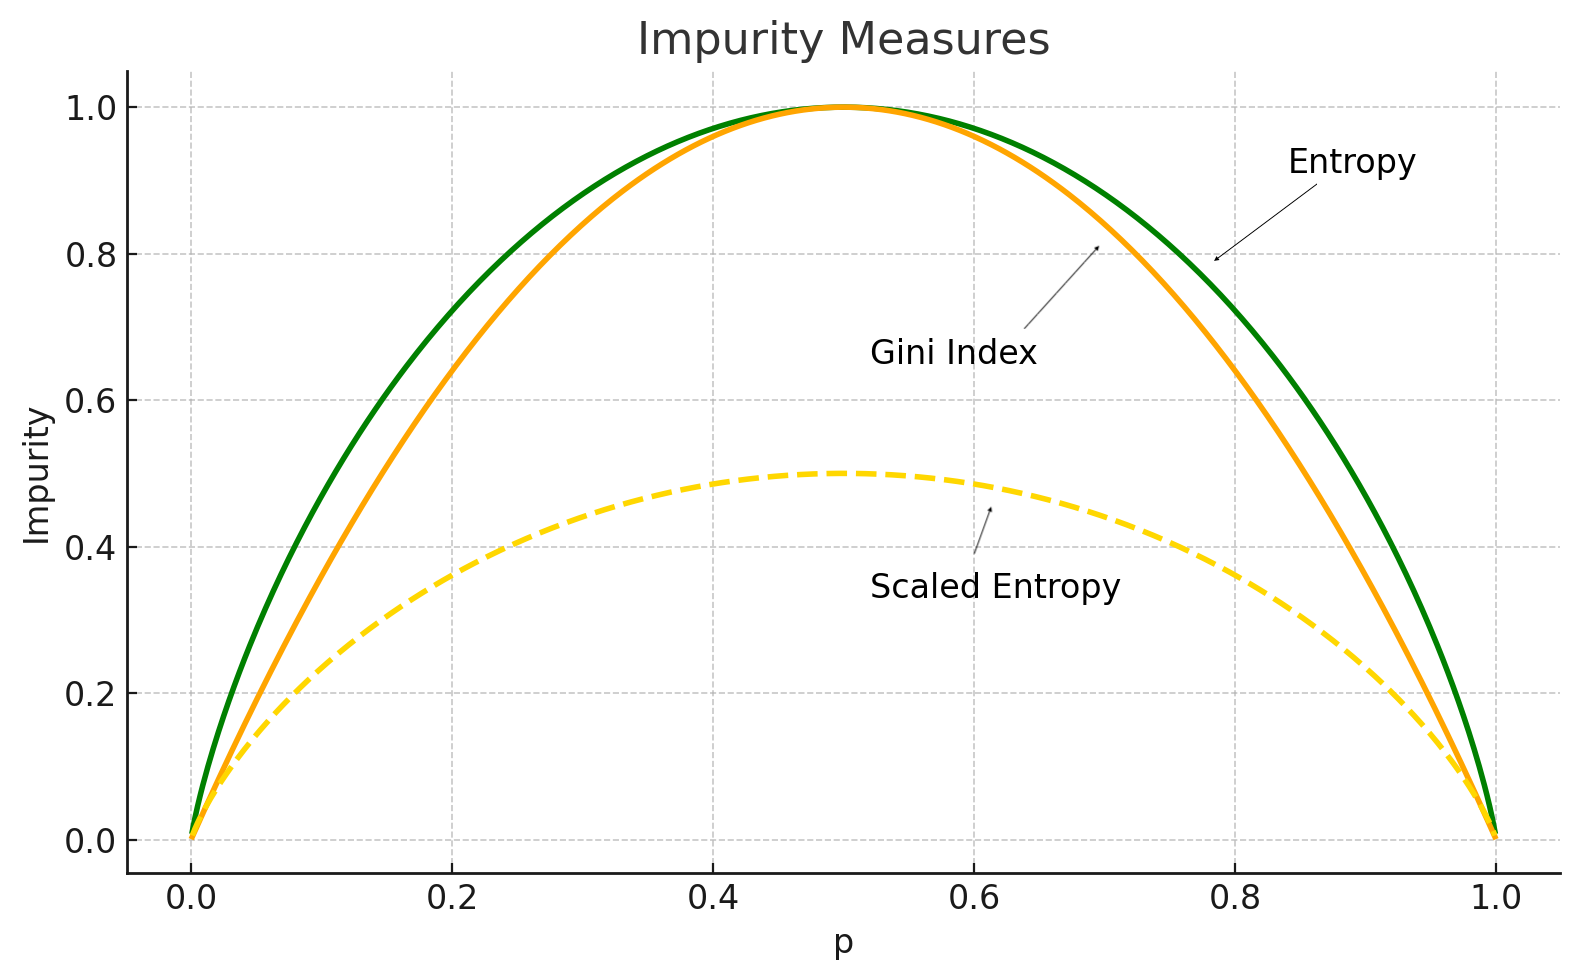
\includegraphics[width=0.5\linewidth]{E-SC-GI.png}
\caption{\label{fig:frog}Impurity Measures in comparison}
\end{figure}

Both Gini Index, Scaled Entropy and Entropy are strictly concave, ensuring a monotonic decrease in impurity after each split, and differentiable, which facilitates numerical optimization during tree construction. 


In particular:
\begin{itemize}
    \item Gini index measures how often a randomly chosen element of a set would be incorrectly labeled if it were labeled randomly and independently according to the distribution of labels in the set. In other word, how mixed the labels are in a node. A lower Gini index indicates a purer node, meaning that all samples in the node are associated with a single target category.

    \item Entropy measures the level of disorder in the labels. Higher entropy means a more diverse set of label, instead lower entropy means a greater homogeneity.

    \item Scaled Entropy is a variation of standard entropy; it presents the same shape but compresses by half. It measures the level of disorder in the label, and it reaches 0.5 - its maximum - when classes are equally represented. Scaled entropy is less sensitive to disorder compared to standard entropy.
\end{itemize}

They follow similar trend but Gini index remains consistently lower than entropy, while scaled entropy follows the same curve as entropy but at a lower scale.

\subsection{Tree Structure (Code)}

The binary decision tree is implemented entirely from scratch; using only single-feature binary tests at each internal node.
A custom TreeNode class represents each node in the tree, storing its splitting condition, child nodes and predicted classes while the node is a leaf. The model includes a section used to determine whether a node represents a leaf or not.

The DecisionTree class contains several parameters which controls the behavior and growth of the model, making it the main class of the prediction model. The class supports the entire training, prediction and visualization metrics of the project. It adopts a flexible configuration through several stopping criteria maximum depth, minimum samples per node, maximum number of leaves, and an impurity threshold. The constructor accepts one of the following impurity measures, Gini index, entropy, or scaled entropy, as the metric for evaluating splits.
The training algorithm builds the tree recursively. For each node, it first checks for stopping condition. If not, it evaluates all possible binary splits across all features \texttt{best\_split}.The best split is determined by the maximum information gain computed.
In other words, tree is developed by repeatedly selecting the best split that maximizes information gain \texttt{information\_gain}, accordingly to the chosen impurity measure.
Single-feature test x[features <= threshold are used to make decision at internal node. Categorical fears are converted into numeric using one-hot encoding, according to the model requirement.
The prediction [predict] traverses the decisione tree for each data sample and continuous until a leaf node is reached. Zero-one loss and accuracy are used to evaluate the model performance. The evaluation metrics are performed both on training and test set in order to assess overfitting, undercutting and how well the model generalizes.

The second section performed a stratified train test and allocates 80% of the data to the training set and 20% of the data to the test set. Since the data set is compesed by several categorical feature, one-hot encoding was applied to both training and test set. In order to avoid inconsistency among training and test set, the test set are reindexed filling any missing value with zero. Class label are encoded to transform them into numerical values which are required by the tree model. 

After data are recalled by main function, tree is initialized through controlled parameters in a static situation. The decision tree is implemented with a maximum depth of 5, a minimum sample split of 5, an entropy threshold of 0.1, iterating for the three splitting criterion. The training process is timed in order to define performance. The training time are relatively high, due to the dataset size and the fact that decision tree is implemented from scratch. Indeed, results highlight the computational cost which are associated with a manual implementation. The training durations for each splitting criterion is:

\begin{table}[H]
\centering
\renewcommand{\arraystretch}{1.3}
\begin{tabular}{|c|c|}
\hline
\textbf{Splitting Criterion} & \textbf{Training Time (sec)} \\
\hline
Gini Index (GI)              & \textbf{59.35}               \\
Entropy (E)                  & \textbf{62.05}               \\
Scaled Entropy (SE)          & \textbf{56.78}               \\
\hline
\end{tabular}
\caption{Training time comparison for different impurity criteria}
\label{tab:training_times}
\end{table}

Moreover, accuracy and zero-one loss are computed to quantify the quality of the prediction. 
The model correctly classifies around 3 out of 4 data points, indicating a solid performance at generalizing without overfitting. Nearly 1 out of 4 data points are incorrectly classified. The highest Test Accuracy is reached by the Gini Index model. Both Entropy and Scaled Entropy yielded identical test accuracy and zero-one loss scores.
Gini Index offers a small advantages in terms of classification accuracy.

\begin{table}[H]
\centering
\renewcommand{\arraystretch}{1.3}
\begin{tabular}{|c|c|c|}
\hline
\textbf{Splitting Criterion} & \textbf{Test Accuracy} & \textbf{Zero-One Loss} \\
\hline
Gini Index (GI)              & \textbf{0.7337}         & \textbf{0.2663}         \\
Entropy / Scaled Entropy     & \textbf{0.7256}         & \textbf{0.2744}         \\
\hline
\end{tabular}
\caption{Test accuracy and zero-one loss for different splitting criteria}
\label{tab:test_accuracy}
\end{table}

Confusion matrix are displayed to provide a visual representation of actual and predicted values.
The model is more accurate when predicting 1 compared to class 0. More specifically, considering the Gini Index model, out of the total actual class 0 samples, 4976 were correctly classified (TN), while 460 were incorrectly predicted as class 1 (FP). For actual class 1, 3986 data points  were correctly predicted (TP), while 2792 were misclassified as class 0 (FN). Similar pattern are recorded for Entropy and Scaled entropy, which yielded identical results.


\begin{figure}[H]
\centering
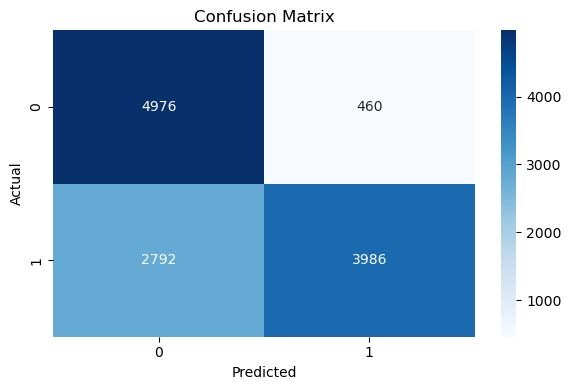
\includegraphics[width=0.5\linewidth]{CM-Gini.png}
\caption{\label{fig:frog}Confusion Matrix - Gini Index}
\end{figure}

\begin{figure}[H]
\centering
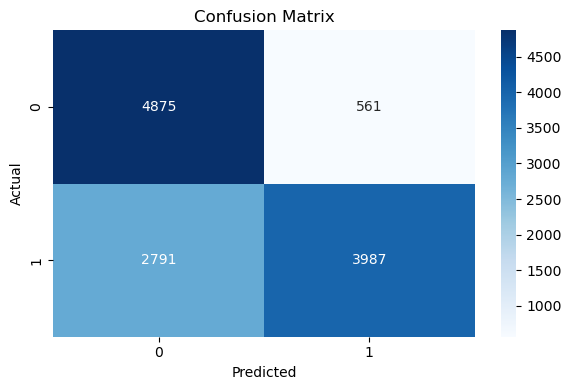
\includegraphics[width=0.5\linewidth]{CM-SE.E.png}
\caption{\label{fig:frog}Confusion Matrix - Entropy and Scaled Entropy}
\end{figure}

Finally, the model produced the decision tree visualization. The binary decision paths, thresholds, and class predictions at leaf nodes are clearly illustrated.

\begin{figure}[H]
\centering
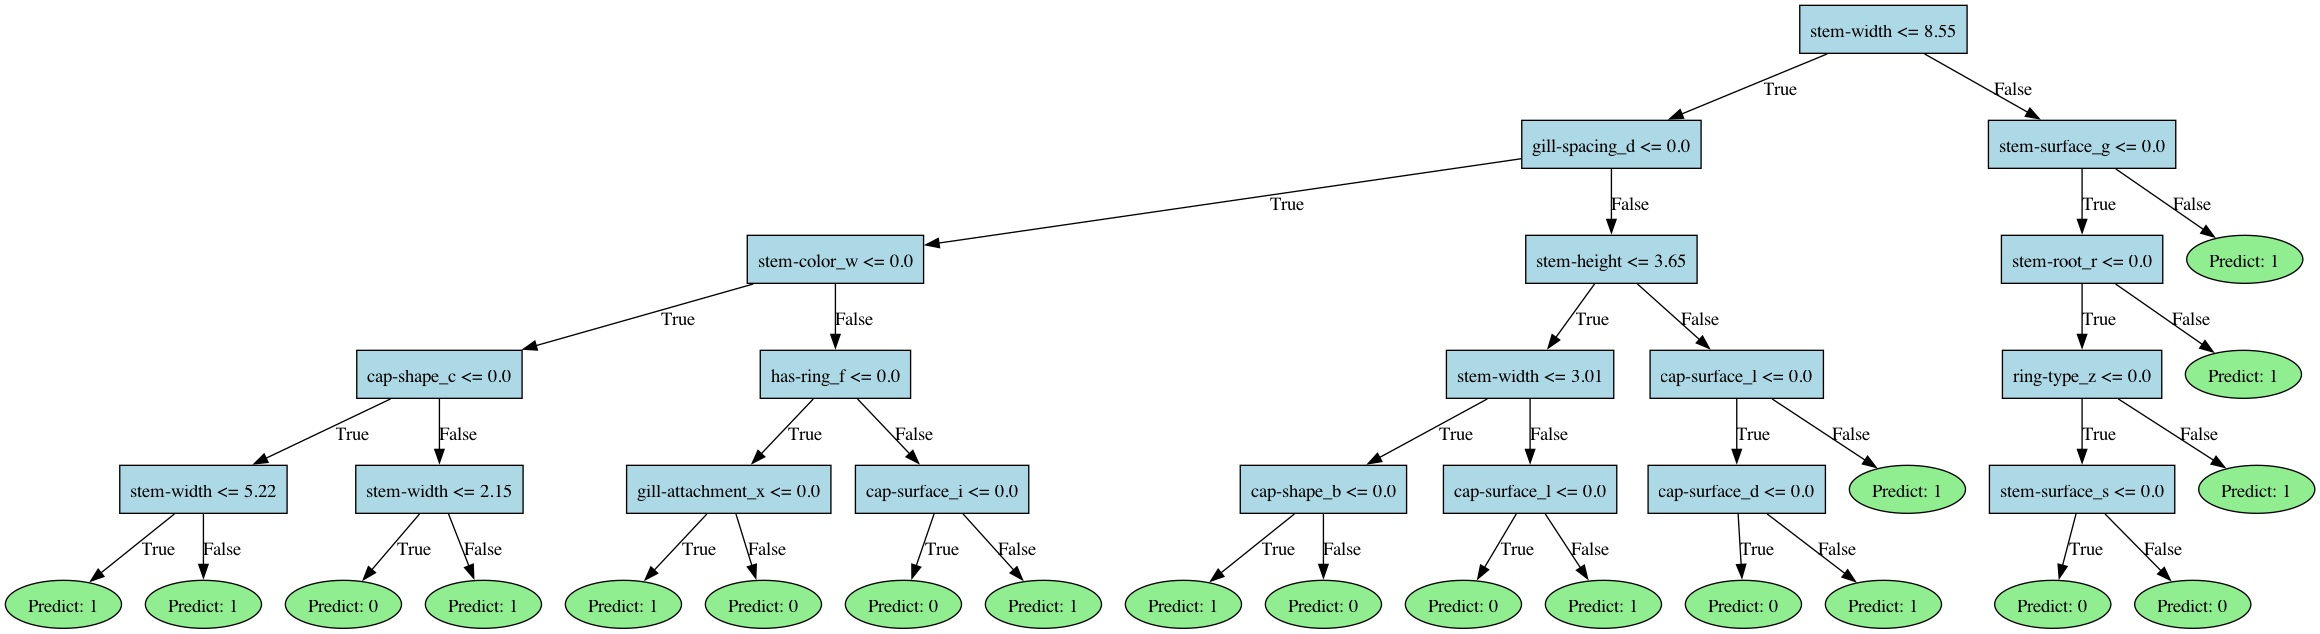
\includegraphics[width=1\linewidth]{Tree_Visual_Gini.jpg}
\caption{\label{fig:frog}Tree Visualization - Gini Index}
\end{figure}


\begin{figure}[H]
\centering
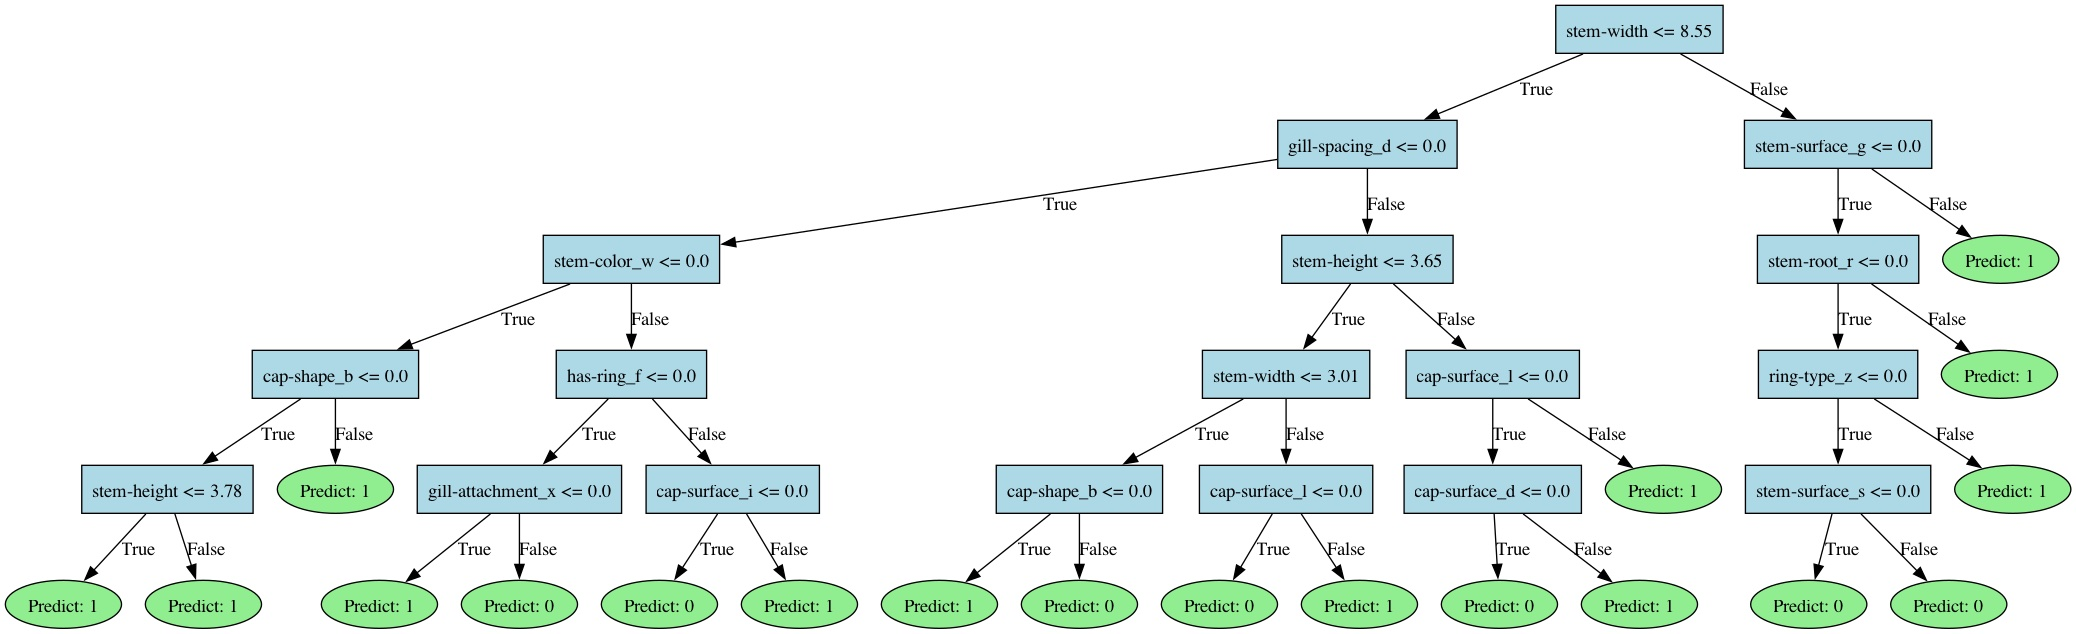
\includegraphics[width=1\linewidth]{Tree_Visual_E.jpg}
\caption{\label{fig:frog}Tree Visualization - Entropy}
\end{figure}

\begin{figure}[H]
\centering
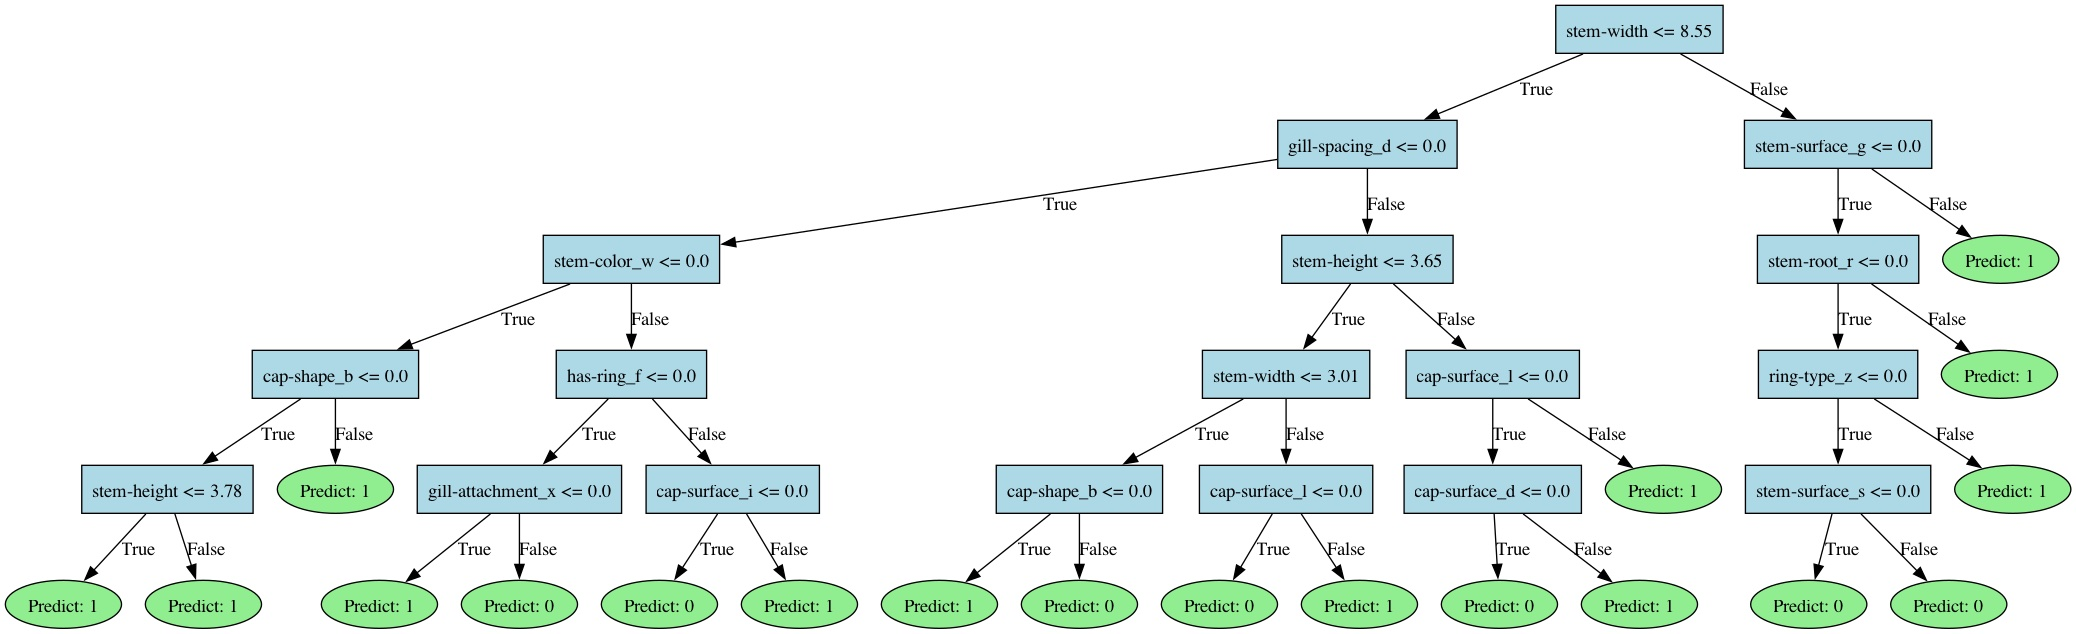
\includegraphics[width=1\linewidth]{Tree_Visual_SE.jpg}
\caption{\label{fig:frog}Tree Visualization - Scaled Entropy}
\end{figure}

The Hyperparameter Tuning procedure is used to evaluate the impact of choosing different splitting criteria and tree depths. In particular, the performance of each model is evaluated across a range of maximum tree depths from 3 to 9 and three different splitting strategies. Each pair of configuration is trained on the dataset and evaluated using accuracy on both the training and test sets. The overfitting gap is used to assess the quality of generalization, which is define as the difference between training and test accuracy.

\begin{table}[H]
\centering
\renewcommand{\arraystretch}{1.2}
\begin{tabular}{|l|c|c|c|c|c|}
\hline
\textbf{Criterion} & \textbf{Max Depth} & \textbf{Train Accuracy} & \textbf{Test Accuracy} & \textbf{Overfitting Gap} \\
\hline
entropy         & 2 & 0.652973 & 0.650565 & 0.002408 \\
entropy         & 3 & 0.681957 & 0.677092 & 0.004865 \\
entropy         & 4 & 0.709631 & 0.710666 & -0.001035 \\
entropy         & 5 & 0.723836 & 0.725561 & -0.001725 \\
entropy         & 6 & 0.740477 & 0.742836 & -0.002359 \\
entropy         & 7 & 0.773432 & 0.775831 & -0.002399 \\
entropy         & 8 & 0.781783 & 0.783363 & -0.001580 \\
entropy         & 9 & 0.797012 & 0.799001 & -0.001990 \\
\hline
gini            & 2 & 0.652973 & 0.650565 & 0.002408 \\
gini            & 3 & 0.681957 & 0.677092 & 0.004865 \\
gini            & 4 & 0.713172 & 0.714508 & -0.001336 \\
gini            & 5 & 0.731471 & 0.733748 & -0.002277 \\
gini            & 6 & 0.748787 & 0.750287 & -0.001499 \\
gini            & 7 & 0.784689 & 0.786393 & -0.001703 \\
gini            & 8 & 0.817173 & 0.816604 & 0.000569 \\
gini            & 9 & 0.839280 & 0.839201 & 0.000079 \\
\hline
scaled\_entropy & 2 & 0.652973 & 0.650565 & 0.002408 \\
scaled\_entropy & 3 & 0.681957 & 0.677092 & 0.004865 \\
scaled\_entropy & 4 & 0.709631 & 0.710666 & -0.001035 \\
scaled\_entropy & 5 & 0.723836 & 0.725561 & -0.001725 \\
scaled\_entropy & 6 & 0.740477 & 0.742836 & -0.002359 \\
scaled\_entropy & 7 & 0.773370 & 0.775831 & -0.002461 \\
scaled\_entropy & 8 & 0.781701 & 0.783363 & -0.001662 \\
scaled\_entropy & 9 & 0.796930 & 0.799001 & -0.002071 \\
\hline
\end{tabular}
\caption{Comparison of train/test accuracy and overfitting gap for different criteria and tree depths.}
\label{tab:accuracy_comparison}
\end{table}


Accuracy is visualized by a matrix where rows represent the splitting criterion, columns represent the maximum tree depth, and cell color intensity encodes test accuracy. The visualization highlights the trade-offs between performance and complexity.


\begin{figure}[H]
\centering

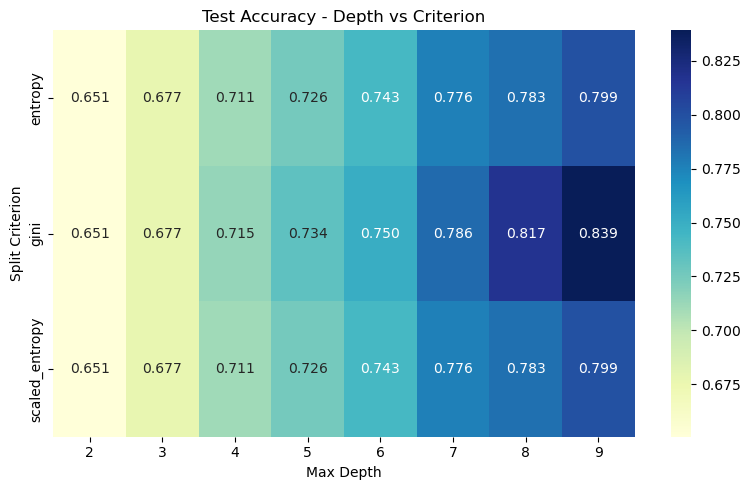
\includegraphics[width=0.7\linewidth]{Hyperparameter Tuning.png}
\caption{\label{fig:frog}Hyperparameter Tuning}
\end{figure}


The figure displays test accuracy as a function of the maximum depth and splitting criterion used in the decision tree. The test accuracy decreases as the maximum depth of the tree decreases, which means that trees of a lower depth are less effective in capturing the complexity of the data set across all three parameters.
Gini - considering all three criterion - outperforms the other two at each level of depth. The best performance is recorded at depth 9 with a test accuracy of 0.839. Both Scaled Entropy and Entropy display identical results; the highest accuracy is reached at 0.799.

The last section of the project aim at selecting the best model configuration considering key criteria: both accuracy and overfitting gap. The best-performing model is the model with the highest test accuracy, which reflects the model’s ability to generalize to unseen data. The most-balanced model, with the lowest absolute overfitting gap, indicates a small distance between training and test performance. The optimal configuration correspond to the decision of using Gini Index as a splitting criterion and a maximum depth of 9. This model recorded a training test accuracy of 0.839201 and an overfitting gap of just 0.000079; showing no signs of overfitting. The same configuration is selected for both analysis, indicating that deeper trees do not compromise the ability to perform well on unseen data.


\section{Conclusion}

The model illustrates that a decision tree which is manually implemented is able to achieve competitive accuracy and generalization performance.

Despite the high computational costs incurred by the model, results demonstrate the quality and effectiveness of implementing a decision tree from scratch. The results highlight that the Gini index is the most accurate parameter, while entropy and scalability performed similarly and but less effectively.
Through systematic hyperparameter tuning, the optimal configuration corresponds to the decision of using Gini Index as a splitting criterion and a maximum depth of 9. This model recorded a training test accuracy of 0.839201 and an overfitting gap of just 0.000079; showing no signs of overfitting and strong generalization capabilities.









\bibliographystyle{alpha}
\bibliography{sample}

\end{document}